\begin{frame}{GUI Layout}{Anordnen von Elementen}
    \begin{itemize}
        \item Bei Nutzen von \texttt{add()} werden Komponenten automatisch platziert
        \item Dies geschieht durch den \textit{Layout Manager}
        \item Manager werden pro Container definiert
        \item Je nach Layout sind ggf. feste "`Slots"' im Container vorhanden
        \item Um Komponente an bestimmter Position zu platzieren wird Überladung von \texttt{add()} verwendet:
        \begin{itemize}
            \item \texttt{add(Component comp, Object constraint)}
            \item \texttt{constraint} definiert Position im Container
        \end{itemize}
    \end{itemize}
\end{frame}

\begin{frame}{GUI Layout}{Größe von Komponenten}
    \begin{itemize}
        \item Komponenten können absolute, minimale, maximale und bevorzugte Größe definieren
        \begin{itemize}
            \item \texttt{setSize(int height, int width)}
            \item \texttt{setMinimumSize(Dimension d)}
            \item \texttt{setMaximumSize(Dimension d)}
            \item \texttt{setPreferredSize(Dimension d)}
        \end{itemize}
        \item Layout Manager \textit{versucht} diese zu beachten
        \item \textit{Müssen} dies jedoch nicht
        \item Insbesondere absolute Größen sind meist gegen das Prinzip von Layout Managern
    \end{itemize}
\end{frame}

\begin{frame}{GUI Layout}{Layout Manager}
    \begin{itemize}
        \item Vorteil von Layout Managern:
        \begin{itemize}
            \item Relative Positionierung von Komponenten kann definiert werden
            \item Vereinfachen erstellen von GUIs
            \item Größe und Position von Komponenten werden automatisch angepasst (Zum Beispiel bei Ändern der Fenstergröße)
        \end{itemize}
    \end{itemize}
\end{frame}

\begin{frame}{BorderLayout}{Grundlegendes (Vgl. \cite{orac:borderlayout})}
    \begin{itemize}
        \item Teil den Container in fünf Bereiche
        \item Diese sind über Konstanten in der \texttt{BorderLayout} Klasse definiert:
        \begin{itemize}
            \item \texttt{PAGE\_START} -- Oberer Bereich (Kopfzeile)
            \item \texttt{PAGE\_END} -- Unterer Bereich (Fußzeile)
            \item \texttt{LINE\_START} -- Linker Bereich zwischen Kopf und Fuß
            \item \texttt{LINE\_END} -- Rechter Bereich zwischen Kopf und Fuß
            \item \texttt{CENTER} -- Mittlerer (Haupt-)bereich
        \end{itemize}
        \item Beispiel: Hinzufügen im \texttt{PAGE\_START} Bereich:
        \begin{itemize}
            \item \texttt{add(button, BorderLayout.PAGE\_START)}
        \end{itemize}        
    \end{itemize}
\end{frame}

\begin{frame}{BorderLayout}{Weitere Eigenschaften (Vgl. \cite{orac:borderlayout})}
    \begin{itemize}
        \item Fokus liegt auf den \texttt{CENTER} Bereich
        \item Dieser nutzt maximal verfügbaren Platz
        \item Alle anderen Bereiche nutzen nur den benötigten Platz
        \item Nicht alle Bereiche müssen genutzt werden
        \item \texttt{PAGE\_START} und \texttt{PAGE\_END} nutzen (sofern vorhanden) immer die volle Breite
        \item Freiräume zwischen Bereichen lassen sich definieren:
        \begin{itemize}
            \item \texttt{setHGap(int)}
            \item \texttt{setVGap(int)}
        \end{itemize}
        \item Standard-Layoutmanager von \texttt{JFrame}
    \end{itemize}
\end{frame}

\begin{frame}{BorderLayout}{Aufgabe}
    \begin{alertblock}{BorderLayout Demo}
    Implementiert eine simple Fensteranwendung, um das Verhalten des \texttt{BorderLayout} kennen zu lernen. Platziert dazu zunächst jeweils einen \texttt{JButton} in
    jedem Bereich. 
    
    Untersucht, wie sich die Größe und Anordnung der Buttons ändert, wenn ihr eine Größe für die Buttons definiert oder wenn ihr einzelne Bereiche im Layout ungenutzt lasst.
    \end{alertblock}
\end{frame}

\begin{frame}{BoxLayout}{Grundlegendes(Vgl. \cite{orac:boxlayout})}
    \begin{itemize}
        \item Ordnet Komponenten entweder vertikal oder horizontal angeordnet
        \item Dafür zwei Konstanten in der \texttt{BoxLayout} Klasse
        \begin{itemize}
            \item \texttt{PAGE\_AXIS} -- Vertikale Anordnung (Als eine "`Spalte"')
            \item \texttt{LINE\_AXIS} -- Horizontale Anordnung (Als eine "`Zeile"')
        \end{itemize}
        \item Komponenten werden dann gemäß \texttt{ComponentAlignment} platziert (Bspw. Linksbündig/Zentriert/Rechtsbündig)
        \item Definierte maximale Größe von Komponenten wird im \texttt{BoxLayout} \textit{immer} respektiert
    \end{itemize}
\end{frame}

\begin{frame}[fragile]{BoxLayout}{Aufgabe}
Entwerft eine Beispielandwendung, in der mehrere Buttons in einem Frame mit dem \texttt{BoxLayout} als Layout Manager. Nutzt folgende Basis um den Layout Manager im \texttt{JFrame()} anzupassen:

\lstset{style=java}
\begin{lstlisting}
JFrame frame = new JFrame();
frame.setSize(300,600);
frame.setLayout(new BoxLayout(window, BoxLayout.PAGE_AXIS));

/*Buttons hinzufügen*/

frame.setVisible(true);
\end{lstlisting}

Experimentiert, was passiert, wenn ihr die Orientierung der einzelnen Komponenten anpasst.
\end{frame}

\begin{frame}{FlowLayout}{(Vgl. \cite{orac:flowlayout})}
    \begin{itemize}
        \item Ist das Standard-Layout von \texttt{JPanel}
        \item Komponenten werden in einer Reihe nebeneinander platziert
        \item Hierbei wird die bevorzugte Größe der Komponenten berücksichtigt
        \item Ist in einer Reihe nicht genug Platz verbleibend für die neue Komponente, so wird eine neue Reihe eingefügt
        \item Positionierung der Reihen kann definiert werden:
        \begin{itemize}
            \item \texttt{BoxLayout.LEFT} -- Linksbündig
            \item \texttt{BoxLayout.RIGHT} -- Rechtsbündig
            \item \texttt{BoxLayout.CENTER} -- Zentriert
            \item \texttt{BoxLayout.LEADING} -- Bündig mit dem Beginn der Container-Orientierung (zB. Links bei Links-nach-Rechts Orientierung)
            \item \texttt{BoxLayout.TRAILING} -- Bündig mit dem Ende der Container-Orientierung (zB. Links bei Rechts-nach-Links Orientierung)
        \end{itemize}
    \end{itemize}
\end{frame}

\begin{frame}{FlowLayout}{Aufgabe}
\begin{alertblock}{}
Entwerft eine simple Fensteranwendung, die über das Hinzufügen mehrerer Buttons mit verschiedener Größe die Funktionsweise des \texttt{FlowLayouts} demonstriert. Ändert hierzu
entweder den LayoutManager des erzeugten \texttt{JFrame} Objekts(Siehe Aufgaben zum BoxLayout) oder fügt ein \texttt{JPanel} hinzu, dem ihr anschließend die Buttons hinzufügt.

Experimentiert mit dem Verhalten des FlowLayouts bei ändern der Fenstergröße.
\end{alertblock}
\end{frame}

\begin{frame}{GridLayout}{Grundlegendes (Vgl. \cite{orac:gridlayout})}
    \begin{itemize}
        \item Rastert den Container in Zeilen und Spalten
        \item Jede "`Zelle"' ist gleichgroß
        \item Komponenten in einer Zelle nehmen die gesamte Zelle ein
        \item Komponenten werden automatisch in die "`nächste"' Zelle hinzugefügt
        \item Initialisierung:
        \begin{itemize}
            \item \texttt{GridLayout()} -- Initialisiert den Container mit einem 1x1 Grid
            \item \texttt{GridLayout(int rows, int cols)} -- Initialisiert das Grid mit der definierten Anzahl an Zeilen und Spalten
        \end{itemize}
        \item Zeilen \textit{oder} Spalten können auf $0$ gesetzt werden $\rightarrow$ Heißt, dass die Anzahl der Zeilen/Spalten dynamisch aus Anzahl der Komponenten ermittelt wird
    \end{itemize}
\end{frame}

\begin{frame}{GridLayout}{Aufgabe}
\begin{alertblock}{}
Entwerft eine Simple Fensteranwendung in der ihr mehrere Komponenten mit dem GridLayout anordnet. Um den Layout Manager zu ändern geht vor wie im Beispielcode zur BoxLayout Aufgabe.

Untersucht, wie sich Anordnung der Komponenten verhält, wenn ihr die Anzahl der Zeilen oder Spalten mit $0$ definiert.
\end{alertblock}
\end{frame}

\begin{frame}{GridBagLayout}{Grundlegendes (Vgl. \cite{orac:gridbaglayout})}
    \begin{itemize}
        \item Ähnlich zum \texttt{GridLayout}
        \item Jedoch flexibler in der Positionierung
        \item Dadurch aber auch komplexer in der Anwendung
        \item Komponenten können in beliebigen Zellen platziert werden
        \item Komponenten können mehrere Zellen einnehmen
        \item Relative Positionierung von Komponenten in den Zellen möglich
    \end{itemize}
\end{frame}

\begin{frame}{GridBagLayout}{Visualisiert}
    \begin{onlyenv}<1|handout:0>
    \begin{figure}
        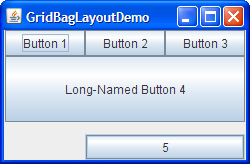
\includegraphics[height=5cm]{graph/gridbag}
        \caption*{\cite{orac:gridbaglayout}}
    \end{figure}
    \end{onlyenv}
    \begin{onlyenv}<2->
    \begin{figure}
        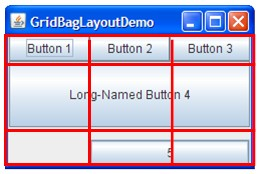
\includegraphics[height=5cm]{graph/gridbagline}
        \caption*{\cite{orac:gridbaglayout}}
    \end{figure}
    \end{onlyenv}
\end{frame}

\begin{frame}{GridBagLayout}{Constraints (Vgl. \cite{orac:gridbaglayout})}
    \begin{itemize}
        \item Platzierung der Komponenten im GridBag wird über \texttt{GridBagConstraints} Objekt definiert
        \item Diese müssen beim hinzufügen von Komponenten mit übergeben werden:
        \begin{itemize}
            \item \texttt{add(Component,GridBagConstraints)}
        \end{itemize}
        \item Für die Constraints lassen sich definieren:
        \item \textbf{\texttt{gridx, gridy}} -- Zeile und Spalte der hinzuzufügenden Komponente. Kann auch als relativ zur zuletzt hinzugefügten Komponente definiert werden
        \item \textbf{\texttt{gridwidth, gridheight}} -- definiert, wie viele Zeilen bzw. Spalten die Komponente einnehmen soll
    \end{itemize}
\end{frame}

\begin{frame}{GridBagLayout}{Constraints (Vgl. \cite{orac:gridbaglayout})}
    \begin{itemize}
        \item \textbf{\texttt{fill}} -- Definiert inwiefern die Komponente den verfügbaren Platz nutzen soll. Kann genutzt werden, um Komponenten horizontal bzw. vertikal auf die Größe der Zelle zu skalieren
        \item \textbf{\texttt{ipadx, ipady, insets}} -- Kann genutzt werden um padding der Komponente zum Rand zu definieren 
        \item \textbf{\texttt{anchor}} -- Definiert die Referenzposition in der Zelle (z.B. links unten, rechts oben etc.)
        \item \textbf{\texttt{weightx, weighty}} -- Wird genutzt um zu bestimmen, wie der gesamt verfügbare Platz auf die einzelnen Zeilen/Spalten verteilt wird. Insbesondere wichtig, wenn die Fenstergröße verändert wird.
    \end{itemize}
\end{frame}

\begin{frame}{GridBagLayout}{Aufgabe}
Experimentiert (wenn ihr wollt) mit dem GridBagLayout und den entsprechenden Constraints. Zur Orientierung könnt die Oracle Tutorial Seite nutzen(Siehe \cite{orac:gridbaglayout})
\end{frame}

\begin{frame}{Layout Manager}{Kombinieren von Layout Managern}
    \begin{itemize}
        \item Komplexe GUIs erfordern nicht zwingend einen komplexen LayoutManager
        \item Da jeder Container Layout Manager selbst definiert können diese kombiniert werden
        \item Heißt: Ein Container wird einem übergeordneten Layout hinzugefügt, verwendet aber für seine eigenen Komponenten einen anderen Manager
        \item Als Basis-Container wird meist ein \texttt{JPanel} verwendet
    \end{itemize}
\end{frame}

\begin{frame}{Layout Manager}{Aufgabe}
\begin{alertblock}{}
Entwerft eine simple GUI Anwendung mit einem BorderLayout. Platziert beliebige Komponenten in den äußeren Bereichen. Platziert im Center Bereich ein \texttt{JPanel}, in dem Komponenten im \texttt{BoxLayout} angeordnet sind.
\end{alertblock}
\end{frame}

\begin{frame}{GUI-Builder}{}
    \begin{itemize}
        \item Alternativ zum "`ausprogrammieren"' der GUI können auch GUI-Builder verwendet werden
        \item Hier werden die Komponenten in einer grafischen Oberfläche platziert
        \item Struktur wird dann meist in XML Format (o.Ä.) übersetzt
        \item Spezieller Layout Manager übernimmt Übersetzung in Code
        \item In IntelliJ integriert
        \item Für Eclipse als Plug-In verfügbar
    \end{itemize}
\end{frame}